\documentclass[12pt]{report}
\usepackage{style}
\usepackage{mathtools}
\author{Aaron Power}
\begin{document}
\chapter{CA1 Usability}
\section{Analysis}
The research question posed is "Is there a significant difference in the mean time taken to find 3 star hotel list between two websites, \textit{discoverireland.ie}, and \textit{discovernorthernireland.com}?". The usability researchers have decided to set their risk of a flase positive decision (\textit{a}) to 5\%.

For the collection of data students, were grouped into pairs, and recorded the time take to display the list of 3 star hotels for each location. A toss of a coin was used to determine which site was searched first. Since, a single parcipant parpicpanted in both tests, a paired t-test is the most suitable experimental design for the study.

<<<<<<< HEAD
\begin{document}
  \begin{acronyms}
    \acrodef*{AST}{Abstract Syntax Tree}
    \acrodef*{CSS}{Cascading StyleSheet}
    \acrodef*{FFI}{Foreign Function Interface}
    \acrodef*{HTML}{HyperText Markup Language}
    \acrodef*{JSON}{JavaScript Object Notation}
    \acrodef*{I18n}{Internationalization and localization}
    \acrodef*{XSLT}{Extensible Stylesheet Language Transformations}
    \acrodef*{XML}{Extensible Markup Language}
  \end{acronyms}
  \maketitle
  \tableofcontents
  \listoffigures
  \listofacronyms
  \chapter{Testing}
  \section{Why write tests?}
Writing tests for a \compiler{} is essential, as the smallest changes in behaviour could cause breaking changes in how the \compiler{}, and might break applications using it as a dependency. If \languageName{} was breaking every application that depended on it, developers would be wary of using it. \languageName{} follows \textit{``semver''}(Semantic Versioning)\cite{semver}. Which is concept of having the version number of the program semantically define when API changes occur. For example \languageName{} version X.Y.Z where X means a major version, changes that would break existing programs are signified here.For example if \languageName{} changed the prefix for variables from ``@'' to ``\%'', the major version would be incremented.Y signifies the minor version, which is changes that extend the program, that also don't break existing programs. For example if \languageName{} added another ``std'' function, the minor version would be incremented. Finally Z represents patch versions, which are reserved for backwards-compatible bug fixes. This system allows for users of \languageName{} to know what to expect when developing with \languageName{} and providing a stable, and predictable way to update their dependencies.
\newpage
Tests also provide a helpful tool for developers who want to develop on, and contribute to \languageName{}. As the tests provide an easy way to test if their code should be merged into \languageName{}. If their code fails the tests it can show the developer that their work needs to be improved, before it can merged, or that they need to rewrite current tests if their code makes a breaking change.

\section{Rust's testing framework.}
The testing was done through Rust's built in testing capabilities. In Rust you can test any module by adding an internal module called \textit{``test''} to the file. All functions with the attribute of \textit{``test''} inside the test module will be run, and any functions that complete are considered to have passed the test, and any test that \textit{``panic!''.}'s(An unexpected error, that results in the termination of the thread or program) is considered to have failed. When a test function has failed any errors from the \textit{``panic!''} are printed out to show where the test failed. To allow for easy testing rust has two macros \textit{``assert!''} which takes a boolean and \textit{``panic!''}'s if the value is false and \textit{``assert\_eq!''} which compares two values, and \textit{``panic!''}'s if they aren't equal.
\newpage
\section{\languageName{} testing.}
Due to being a library/\compiler{} tests involving users such as user acceptance testing or usability testing weren't suitable. This is due to the the project having a very niche target, and a high learning curve. As the required knowledge consists of knowledge of \acro{HTML}, \acro{CSS}, the concept of a templating language, and knowledge of Rust. Instead the focus of testing is in types that allow \languageName{} to be a great and stable library/\compiler{}, such as unit tests, end-to-end tests, and regression tests. Performance testing was considered, but due to the lack of pre-existing templating languages built in Rust during the development of \languageName{} there wasn't an opportunity to perform those types of tests.
\subsection{Unit tests.}
Unit testing is one of the smallest form of testing, typically only testing a single module, function, or struct. \languageName{} has most of unit tests on the ``Lexer'' struct. As if the lexer's output isn't what is expected it will have a chain reaction into the parser, and code generation stages which rely on perfect lexer output. Most of the lexer's unit tests are focused on ensuring that certain characters are correctly interpreted as symbols. That unnecessary whitespace is removed, and that when characters are transformed into lexemes that their positions, are the as they were in the source code. Unit tests weren't performed on the parser, or codegen structs, due to the difficulty of replicating the data structures used, as they were designed around being created, and modified through those stages not to be directly instantiated with existing data. See example Figure~\ref{fig:exampleTest}.

\begin{figure}[!hbtp]
    \begin{minted}{rust}
        #[cfg(test)]
        mod test {
            #[test]
            fn dollar_operator() {
                let lexer = Lexer::new("$");

                assert_eq!(lexer.output(), vec![Symbol(0, Dollar)]);
            }
        }
    \end{minted}
    \caption{An example of a test function.}
    \label{fig:exampleTest}
\end{figure}

\newpage
\subsection{End-to-end tests.}
The majority of tests done were end-to-end and regression tests, as these types of tests can encompass much more scope of the program, and accurately inform how the \compiler{} actually compiled a source file. A lot of the tests were written in such a way to actually function as both types of tests. The tests were run using the \textit{``Template''} API as this API is what developers using \languageName{} would use to render their templates. The template API also goes through all the stages of compilation, bubbling up any errors generated. The errors are also written as so that it will clearly differentiate the location of the error, showing if it was from the parser, code generator, or the template itself. On completion of that task without any \textit{``panic!''}'s the end-to-end test is considered a pass.
\newpage
\subsection{Regression tests.}
The output of the end-to-end test is then used in the regression tests, being compared to an expected \acro{HTML} version. There is a version of this type of test for each feature(elements, components, variables, localisation, functions), and also for each ``std'' function provided. These tests provide regression in case any of behaviour change within those features, if the failing test is deemed to be failing due to change(Where the failure is due to intentional behaviour change, and not a bug) the major version of \languageName{} would be incremented, allowing for developer's using the older versions to maintain their code-bases. This also allows developer's to decide when they are comfortable migrating to the latest version.

\begin{figure}[!hbtp]
    \Large{\textbf{Test code(Rust).}}\normalsize{}
    \begin{minted}{rust}
        const BASIC: &'static str = "<!DOCTYPE html><html><body><p>\ 
        Hello World!</p></body></html>";
        #[test]
        fn element() {
            assert_eq!(Template::load("./tests/element.polly")
                           .unwrap()
                           .no_locales()
                           .unwrap_render("en"),
                       BASIC);
        }
    \end{minted}
    \Large{\textbf{Source code(Polly).}}\normalsize{}
    \begin{verbatim}
        /!DOCTYPE(html)
        /html{
            /body {
                /p{Hello World!}
            }
        }
    \end{verbatim}
    \caption{An example of an end-to-end, and regression test.}
\end{figure}
  \printbibliography
\end{document}
=======
\section{Data}
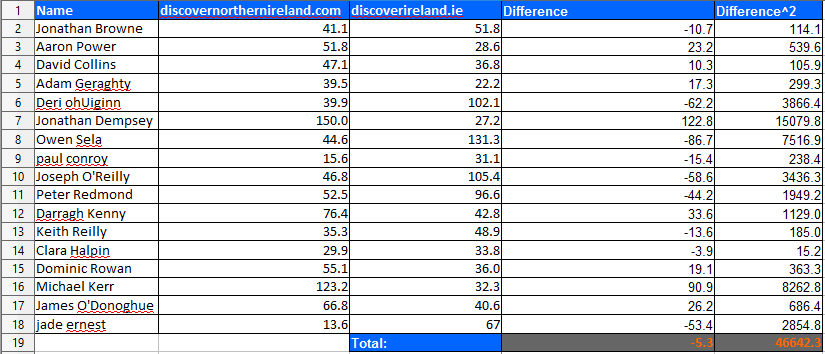
\includegraphics{exceltable.png}
\section{Formulas}
\begin{align*}
     d &= \text{number of participants.} \\
     \overline{d} &= \text{average difference.} \\
     S^2_d &= \frac{\sum d_{i^2} - \frac{(\sum d_i)^2}{d}}{d-1} \\
     t &= \frac{\overline{d} - 0}{\frac{sd}{\sqrt{d}}} \\
\end{align*}

\section{Solution}
\subsection{Hypothesis}
The null hypothesis can be expressed formally as:
\[ H_o: u_1 - u_2 = 0 \text{ or } u_1 = u_2 \text{ for all 17 observations.}\]
The alternative hypothesis is
\[H_1: u_1 \neq u_2\]

\subsection{Calculate the test statistic}

\[t = \frac{\overline{d} - 0}{\frac{S_d}{\sqrt{d}}}\]
with \(d - 1\) degrees of freedom

\begin{align*}
d &= 17\\
\overline{d} &= \frac{-5.3}{17} = 0.3117\\
S^2_d &= \frac{46642.3 - \frac{-5.3^2}{17}}{16}\\
S_d &= \sqrt{\frac{46642.3 - \frac{-5.3^2}{17}}{16}}
= \sqrt{\frac{46642.3 - 1.6523}{16}}
= \sqrt{\frac{46640.6476}{16}}
= \sqrt{2915.0404}
= 53.9911\\
t &= \frac{0.3117}{\frac{53.9911}{\sqrt{17}}}
= \frac{0.3117}{4.1231}
= 0.07559\\
\end{align*}


\subsection{Make the decision}
The \textbf{t} with 16 degrees of freedom and having cumulative probabilities of 97.5\% (as the test is two-tailed with \(a\) = 0.05) the critical values of \(\pm2.120\) are obtained.  As the calculated \textbf{t} is 0.07559 falls well outside the critical region(s) we fail to reject the hypothesis of no difference in load times of the websites. It is important to note that as the sample size is reasonably small, the type 2 error (or false negative) rate could be high.  This can be reduced by conducting a larger study.
larger study. 
\end{document}
>>>>>>> parent of 7370882... finished thesis
